% +--------------------------------------------------------------------+
% | Sample Chapter 2
% +--------------------------------------------------------------------+

\cleardoublepage

% +--------------------------------------------------------------------+
% | Replace "This is Chapter 2" below with the title of your chapter.
% | LaTeX will automatically number the chapters.
% +--------------------------------------------------------------------+

\chapter{Estado del arte}
\label{makereference2}
En esta sección de la memoria procederemos a describir las tecnologías que hemos implementado
en nuestro trabajo, tales como la \textbf{realidad aumentada}, las distintas \textbf{fuentes de información}, 
\textbf{técnicas de recomendación}, junto a un análisis de la \textbf{competencia}.
\section{Realidad Aumentada}
\label{makereference2.1}


Encontramos muchas definiciones distintas, nosotros compartiremos la siguiente:


\begin{quote}
``
La \textbf{realidad aumentada} es el término que se 
usa para describir al conjunto de tecnologías que permiten que un usuario visualice parte de mundo real a través de un dispositivo tecnológico 
con información gráfica añadida por éste dispositivo. Este dispositivo o conjunto de dispositivos, añaden información virtual a la información 
física ya existente, es decir, una parte sintética virtual a la real.
''\cite{rawikipedia}
\end{quote}


\begin{figure}[htb]
    \centering
    \makebox[0pt][c]{%
    \begin{minipage}[b]{0.5\linewidth}
    \centering
      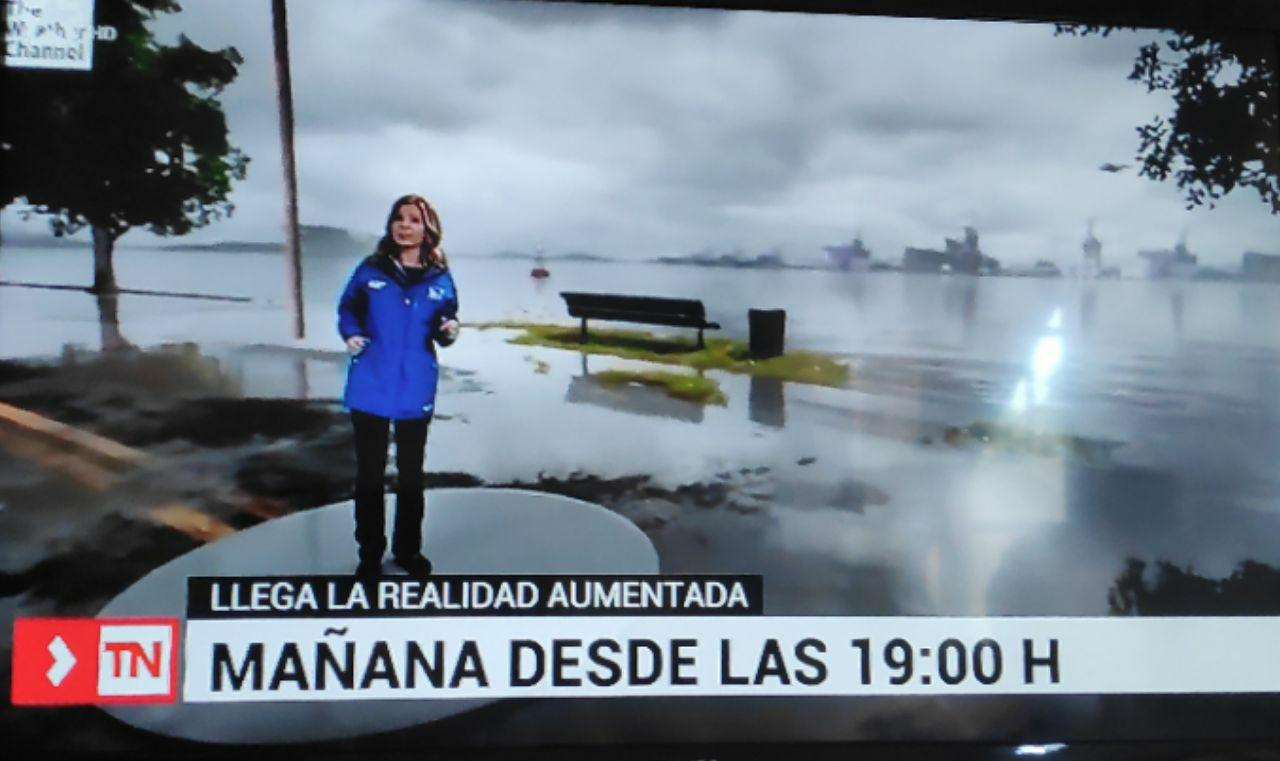
\includegraphics[scale=0.2]{figures/chapter-2/televisionAR-1.jpg}
      \caption{Telemadrid anuncia el uso de RA en las elecciones de 2019}
    \label{sva}
    \end{minipage}%
    \hspace{0.3cm}
    \begin{minipage}[b]{0.5\linewidth}
    \centering
     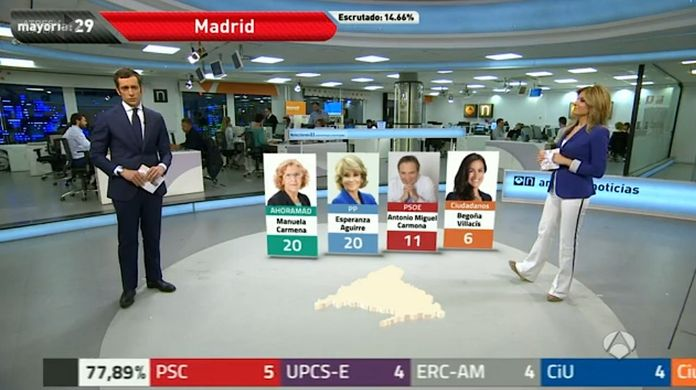
\includegraphics[scale=0.3]{figures/chapter-2/televisionAR-3.jpg}
      \caption{Antena 3 usa RA para las elecciones del ayuntamiento de Madrid}
    \label{svb}
    \end{minipage}%
    }%
\end{figure}


La \textbf{realidad aumentada} se aplica a diversas áreas como seguridad, logística, sanidad, ocio, etc...
 Se pude aplicar a tantas disciplinas como podamos imaginar y no sólo se ha convertido en una herramienta útil si no que es una tecnología atractiva
 y además signo de modernidad. Por estas razones actualmente vemos ejemplos como el de las televisiones que compiten por aplicarla a sus programas
 y presumir de dar el mejor servicio a sus espectadores como vemos en las figuras 2.1 y 2.2. Con esta situación podemos por tanto estar de acuerdo
 en que es una tecnología en auge actualmente. 


Los \textbf{smartphones} son los dispositivos que más interaccionan con esta tecnología, ya que prácticamente todas las personas poseen uno
 y están dotados de un amplio abanico de sensores necesarios para su correcto funcionamiento. Por esto elegimos este tipo de dispositivos para nuestro
 proyecto para los cuales esta tecnología nos permite añadir un valor importante a nuestra aplicación, consideramos que el grueso de nuestro proyecto se
 centra en ella. Los casos de uso más importantes de nuestra aplicación usarán la \textbf{realidad aumentada} para proveer al usuario de información adicional
 y de gran relevancia de las imágenes que reconozca, ya sean carteles de películas o caras de usuarios que usen la aplicación.


\subsection{Tecnologías actuales}
\label{makereference2.1.1}
\paragraph{ARCore\cite{arcore}:}
Plataforma creada por Google para desarrollar aplicaciones de
 realidad aumentada con soporte para Android, Android NDK, iOS,
 Unity y Unreal Engine. Aunque las funcionalidades que se ofrecen
 para iOS y Unity for iOS se limitan a Cloud Anchors. Los anchors
 son herramientas que permiten que objetos virtuales aparezcan en un lugar
 captado por la cámara de nuestro dispositivo estos son compartidos
 en la nube para que multitud de dispositivos disfruten de la misma
 experiencia, los dispositivos con iOS podrán usarlos utilizando ARKit.

Tiene una curva de aprendizaje media y con su versión 1.5 demuestra una
 estabilidad interesante respecto a su reciente creación. Cabe destacar
 que no todos los dispositivos son compatibles, esto depende de que las
 empresas que desarrollan estos dispositivos cumplan unos requisitos
 para asegurar que la experiencia con ARCore es la adecuada y de la
 versión del sistema operativo. Para más información, consultar la información
 provista por Google en el siguiente enlace \url{https://developers.google.com/ar/discover/supported-devices}.

ARCore usa tres características a través de la cámara del dispositivo:
 \begin{itemize}  
     \item {\bf Motion tracking} permite al dispositivo entender y rastrear la posición relativa del mundo.
     \item {\bf Environmental understanding} permite al dispositivo detectar el tamaño y localización de todos los tipos de superficies.
     \item {\bf Light estimation} permite al dispositivo estimar las condiciones de luz del entorno actual.
 \end{itemize}

\paragraph{ARKit:}
Podemos utilizar experiencias de realidad aumentada persistente, compartirlas entre distintos dispositivos iOS,
 detecta imágenes 2D incluso en movimiento y objetos 3D.

\paragraph{Wikitude:}
Kit de desarrollo para realidad aumentada con soporte para Android, iOS, Unity, Cordova, Xamarin (mala
 documentación y versiones obsoletas), Titanium, React Native.
Su licencia es de pago, aunque hay versiones limitadas gratuitas.
Utiliza ARCore o ARKit cuando los dispositivos lo soportan y en caso contrario utiliza tecnología de Wikitude
 para que el número de dispositivos compatibles sea mayor. 

\paragraph{Vuforia:}
Kit de desarrollo para realidad aumentada con soporte para Android, iOS, UWP y Unity.
Software de pago solo permite usarse gratis para pruebas.

\paragraph{ViroReact:}
Plataforma para construir aplicaciones con realidad aumentada usando React Native.
 Utiliza ARKit y ARCore para dotar a las aplicaciones de una experiencia de Realidad Aumentada sin
 utilizar código distinto y con una curva de aprendizaje fácil. Al basarse en React
 Native que no tiene versión estable provoca problemas con las versiones de dependencias,
 configuraciones tediosas y largas compilaciones.
Es un software privativo gratuito.

\paragraph{Expo AR:}
API que permite crear aplicaciones en React Native utilizando ARKit únicamente.
Está en una fase muy inicial.

\section{Análisis de la competencia}
\label{makereference2.2}
\begin{flushleft}
    Consideramos que la aplicación que hemos diseñado consta de dos partes claramente diferenciadas (la parte de \textbf{Realidad Aumentada} 
    y la parte de \textbf{Recomendación y gestión} de películas), además, pensamos que existen distintos tipos de competencia dependiendo de cada una de ellas.
     \begin{itemize}  
         \item En la parte de recomendación y gestión de películas, compite claramente con aplicaciones como \textbf{IMDB} o \textbf{MovieBase}. 
         Estas aplicaciones proporcionan, herramientas para guardar películas y recomendar éstas a los usuarios en función de sus gustos. Estas funcionalidades son 
         muy parecidas a las que nosotros hemos decidido proporcionar a nuestros usuarios, con la diferencia que nuestra aplicación, además de las funcionalidades anteriormente 
         mencionadas, permite realizar más acciones sobre las películas como crear planes con amigos.
        \item A diferencia de la parte de recomendación y gestión en donde hay una gran variedad de aplicaciones que ofrecen servicios parecidos a los nuestros, únicamente hemos 
        encontrado una aplicación (\textbf{Paramount AR+}) que ofrezca servicios parecidos a los nuestros relacionados con Realidad Aumentada. Según las especificaciones de la aplicación permite identificar pósteres y 
        mostrar información sobre la película detectada, servicio muy parecido al que nosotros hemos proporcionado. 
    \end{itemize}
    Para intentar alejarnos de esta competencia, hemos decidido unir ambas funcionalidades en una aplicación y, además, proporcionar al usuario más funcionalidades como escanear una aplicación con Realidad Aumentada, 
    ver su información y añadirla a un plan con amigos para ver dicha película. Para funcionalidades como ésta y otras en las que unimos la realidad aumentada con la recomendación de películas y gestión de planes no hemos encontrado actualmente ninguna aplicación que proporcione estos servicios.
    \\
    Además, una funcionalidad nuestra aplicación proporciona y no hemos encontrado otra que lo haga es la gestión de amigos con Realidad Aumentada. 
    Como que al enfocar con la cámara a un amigo y que en la misma pantalla de realidad Aumentada muestre visualmente la información de los tres planes activos que tiene mi amigo que más podrían gustarme y cuanto se estima que me gustaría ese plan.
    
\end{flushleft}
\newpage
\section{Fuentes de información}
\label{makereference2.3}
Como nuestra aplicación muestra información sobre las películas que se recomiendan y que los usuarios han guardado, hemos
tenido que investigar de que página web podríamos obtener estos datos tan relevantes.
\paragraph{IMDB:}
Nos decidimos por usar la página web de \textbf{IMDB}: \url{https://www.imdb.com/} para conseguir las valoraciones, resúmenes, nombre del director,
género y país de las películas, entre otros datos, debido a que consideramos que es de las webs más usadas entre los cinéfilos y posibles 
usuarios de nuestra aplicación.

\section{Técnicas de recomendación}
\label{makereference2.4}
En nuestra aplicación, tenemos los siguientes datos para nuestro sistema de recomendación: \textbf{Información de usuarios}, \textbf{Información de películas} y \textbf{Valoraciones de los usuarios a las películas}.
Entre los distintos tipos de sistemas de recomendación, vamos a destacar dos, pues son los que mejor se asemejan a nuestra situación.

\begin{itemize}
    \item \textbf{Filtrado Colaborativo:} Este sistema de recomendación se basa en buscar usuarios que tienen preferencias similares. Si a un individuo le ha gustado una película, entonces le recomendará las películas que le gustaron a otros usuarios a los que también les gustó esta.
    \item \textbf{Filtrado basado en el contenido:} Como indica su nombre, está basado en su contenido, si a alguien le gusta una película, se le va a recomendar otra que es parecida.
\end{itemize} 

\begin{figure}[H]
    \centering
    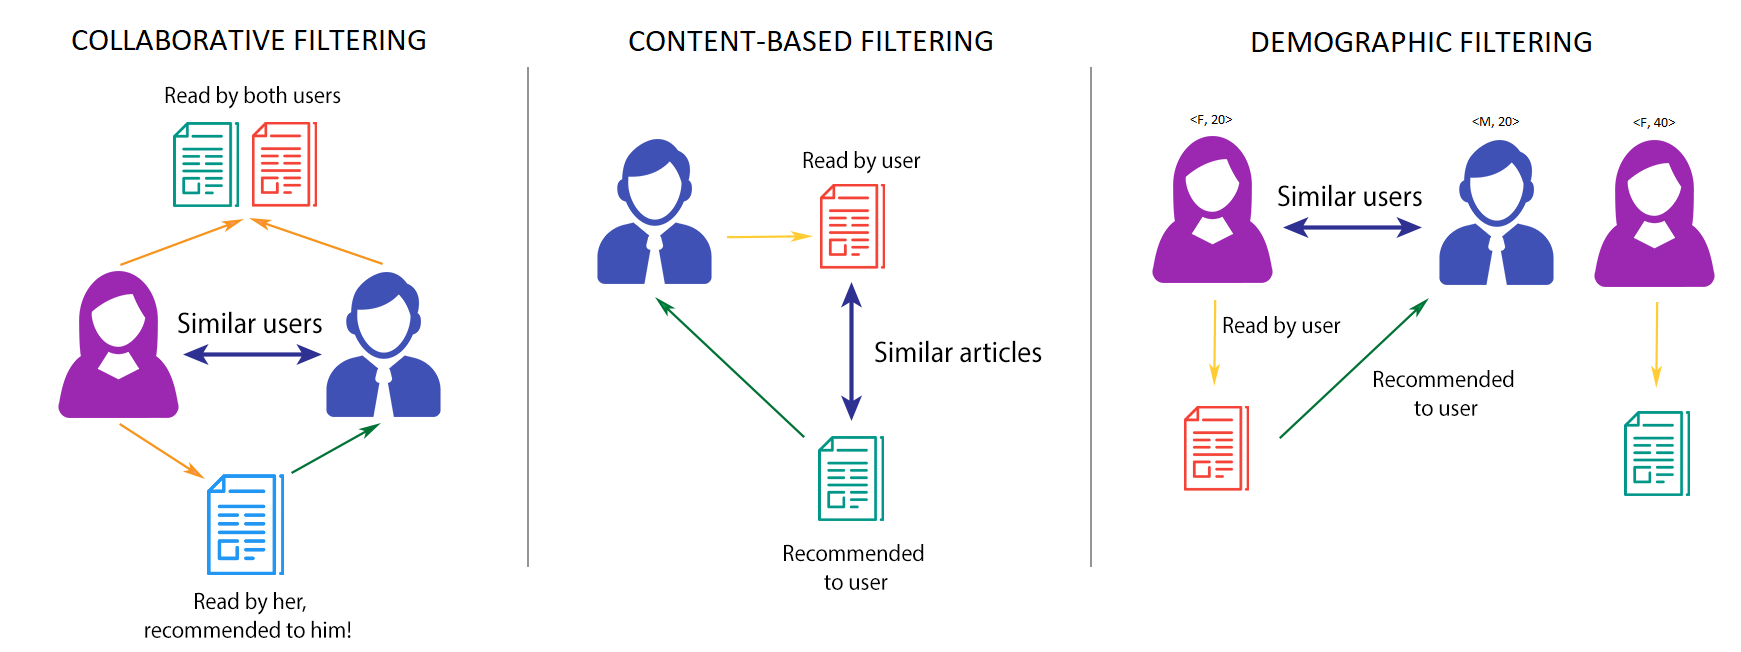
\includegraphics[width=3in, angle=0]{figures/chapter-2/recommendation_systems.png}
    \caption{Tipos de sistemas de recomendación}
\end{figure}

Finalmente decidimos usar para la aplicación el sistema de \textbf{Filtrado Colaborativo} por los siguientes motivos:

\begin{itemize}
    \item Tenemos valoraciones de usuarios a películas que podemos aprovechar, ya que es una de las acciones que puede realizar un usuario y se aprovecha para recolectar los datos.
    \item Hemos conseguido un archivo csv de unas 200000 valoraciones de usuarios a películas con sus respectivos títulos. Por lo que sólo tendríamos que crear usuarios ficticios para conseguir una base de datos inicial.
    \item Para usar el filtrado basado en el contenido tenemos que diseñar muy bien los datos de cada una de las entidades, además de aplicar los pesos de importancia a los atributos para en un futuro aplicar el sistema.  
\end{itemize} 

